\documentclass[conference]{IEEEtran}
\IEEEoverridecommandlockouts
\usepackage{cite}
\usepackage{amsmath,amssymb,amsfonts,amsthm}
\usepackage{graphicx}
\usepackage{textcomp}
\usepackage{xcolor}
\usepackage{booktabs}
\usepackage{url}
\graphicspath{{figures/}}
\setlength{\textfloatsep}{7pt plus 2pt minus 2pt}
\setlength{\dbltextfloatsep}{7pt plus 2pt minus 2pt}
\setlength{\floatsep}{6pt plus 2pt minus 2pt}
\setlength{\dblfloatsep}{6pt plus 2pt minus 2pt}
\newcommand{\nSeeds}{20}
\newcommand{\nRuns}{1000}
\newcommand{\nMethods}{10}
\newcommand{\meanlowstaticequal}{4.45}
\newcommand{\meanlowstaticequalLL}{1.3}
\newcommand{\meanlowstaticequalEMBB}{7.4}
\newcommand{\meanlowstaticequalUtil}{47.2}
\newcommand{\meanlowreactiveprop}{0.83}
\newcommand{\meanlowreactivepropLL}{1.6}
\newcommand{\meanlowreactivepropEMBB}{0.1}
\newcommand{\meanlowreactivepropUtil}{50.0}
\newcommand{\meanlowmaxweight}{0.90}
\newcommand{\meanlowmaxweightLL}{1.8}
\newcommand{\meanlowmaxweightEMBB}{0.1}
\newcommand{\meanlowmaxweightUtil}{50.0}
\newcommand{\meanlowqueueaware}{0.52}
\newcommand{\meanlowqueueawareLL}{0.7}
\newcommand{\meanlowqueueawareEMBB}{0.3}
\newcommand{\meanlowqueueawareUtil}{50.0}
\newcommand{\meanlowpointforecast}{0.27}
\newcommand{\meanlowpointforecastLL}{0.3}
\newcommand{\meanlowpointforecastEMBB}{0.2}
\newcommand{\meanlowpointforecastUtil}{50.1}
\newcommand{\meanlowfixedquantile}{0.34}
\newcommand{\meanlowfixedquantileLL}{0.1}
\newcommand{\meanlowfixedquantileEMBB}{0.5}
\newcommand{\meanlowfixedquantileUtil}{50.0}
\newcommand{\meanlowproposedwindow}{0.25}
\newcommand{\meanlowproposedwindowLL}{0.4}
\newcommand{\meanlowproposedwindowEMBB}{0.1}
\newcommand{\meanlowproposedwindowUtil}{50.1}
\newcommand{\meanlowproposed}{0.15}
\newcommand{\meanlowproposedLL}{0.2}
\newcommand{\meanlowproposedEMBB}{0.1}
\newcommand{\meanlowproposedUtil}{50.1}
\newcommand{\meanlowproposedcal}{0.17}
\newcommand{\meanlowproposedcalLL}{0.2}
\newcommand{\meanlowproposedcalEMBB}{0.1}
\newcommand{\meanlowproposedcalUtil}{50.1}
\newcommand{\meanloworacle}{0.07}
\newcommand{\meanloworacleLL}{0.0}
\newcommand{\meanloworacleEMBB}{0.1}
\newcommand{\meanloworacleUtil}{50.2}
\newcommand{\meanmoderatestaticequal}{9.65}
\newcommand{\meanmoderatestaticequalLL}{4.8}
\newcommand{\meanmoderatestaticequalEMBB}{14.2}
\newcommand{\meanmoderatestaticequalUtil}{57.5}
\newcommand{\meanmoderatereactiveprop}{4.11}
\newcommand{\meanmoderatereactivepropLL}{7.6}
\newcommand{\meanmoderatereactivepropEMBB}{0.8}
\newcommand{\meanmoderatereactivepropUtil}{63.5}
\newcommand{\meanmoderatemaxweight}{4.85}
\newcommand{\meanmoderatemaxweightLL}{9.3}
\newcommand{\meanmoderatemaxweightEMBB}{0.7}
\newcommand{\meanmoderatemaxweightUtil}{63.3}
\newcommand{\meanmoderatequeueaware}{4.24}
\newcommand{\meanmoderatequeueawareLL}{3.3}
\newcommand{\meanmoderatequeueawareEMBB}{5.1}
\newcommand{\meanmoderatequeueawareUtil}{62.2}
\newcommand{\meanmoderatepointforecast}{3.23}
\newcommand{\meanmoderatepointforecastLL}{1.8}
\newcommand{\meanmoderatepointforecastEMBB}{4.6}
\newcommand{\meanmoderatepointforecastUtil}{62.7}
\newcommand{\meanmoderatefixedquantile}{4.35}
\newcommand{\meanmoderatefixedquantileLL}{0.6}
\newcommand{\meanmoderatefixedquantileEMBB}{7.9}
\newcommand{\meanmoderatefixedquantileUtil}{61.3}
\newcommand{\meanmoderateproposedwindow}{2.57}
\newcommand{\meanmoderateproposedwindowLL}{2.0}
\newcommand{\meanmoderateproposedwindowEMBB}{3.1}
\newcommand{\meanmoderateproposedwindowUtil}{63.4}
\newcommand{\meanmoderateproposed}{2.15}
\newcommand{\meanmoderateproposedLL}{1.4}
\newcommand{\meanmoderateproposedEMBB}{2.8}
\newcommand{\meanmoderateproposedUtil}{63.6}
\newcommand{\meanmoderateproposedcal}{2.17}
\newcommand{\meanmoderateproposedcalLL}{1.4}
\newcommand{\meanmoderateproposedcalEMBB}{2.9}
\newcommand{\meanmoderateproposedcalUtil}{63.6}
\newcommand{\meanmoderateoracle}{1.62}
\newcommand{\meanmoderateoracleLL}{0.0}
\newcommand{\meanmoderateoracleEMBB}{3.1}
\newcommand{\meanmoderateoracleUtil}{63.7}
\newcommand{\meanhighstaticequal}{15.46}
\newcommand{\meanhighstaticequalLL}{9.8}
\newcommand{\meanhighstaticequalEMBB}{20.8}
\newcommand{\meanhighstaticequalUtil}{65.8}
\newcommand{\meanhighreactiveprop}{9.20}
\newcommand{\meanhighreactivepropLL}{14.7}
\newcommand{\meanhighreactivepropEMBB}{4.0}
\newcommand{\meanhighreactivepropUtil}{74.7}
\newcommand{\meanhighmaxweight}{11.54}
\newcommand{\meanhighmaxweightLL}{20.6}
\newcommand{\meanhighmaxweightEMBB}{2.9}
\newcommand{\meanhighmaxweightUtil}{74.1}
\newcommand{\meanhighqueueaware}{11.03}
\newcommand{\meanhighqueueawareLL}{5.2}
\newcommand{\meanhighqueueawareEMBB}{16.5}
\newcommand{\meanhighqueueawareUtil}{69.3}
\newcommand{\meanhighpointforecast}{9.70}
\newcommand{\meanhighpointforecastLL}{3.1}
\newcommand{\meanhighpointforecastEMBB}{16.0}
\newcommand{\meanhighpointforecastUtil}{70.1}
\newcommand{\meanhighfixedquantile}{11.76}
\newcommand{\meanhighfixedquantileLL}{0.9}
\newcommand{\meanhighfixedquantileEMBB}{22.0}
\newcommand{\meanhighfixedquantileUtil}{67.0}
\newcommand{\meanhighproposedwindow}{8.72}
\newcommand{\meanhighproposedwindowLL}{3.7}
\newcommand{\meanhighproposedwindowEMBB}{13.5}
\newcommand{\meanhighproposedwindowUtil}{71.5}
\newcommand{\meanhighproposed}{8.00}
\newcommand{\meanhighproposedLL}{3.4}
\newcommand{\meanhighproposedEMBB}{12.3}
\newcommand{\meanhighproposedUtil}{72.2}
\newcommand{\meanhighproposedcal}{8.14}
\newcommand{\meanhighproposedcalLL}{2.9}
\newcommand{\meanhighproposedcalEMBB}{13.1}
\newcommand{\meanhighproposedcalUtil}{71.9}
\newcommand{\meanhighoracle}{6.89}
\newcommand{\meanhighoracleLL}{0.0}
\newcommand{\meanhighoracleEMBB}{13.4}
\newcommand{\meanhighoracleUtil}{72.3}
\newcommand{\meanoverloadburstsstaticequal}{19.15}
\newcommand{\meanoverloadburstsstaticequalLL}{13.4}
\newcommand{\meanoverloadburstsstaticequalEMBB}{24.2}
\newcommand{\meanoverloadburstsstaticequalUtil}{67.9}
\newcommand{\meanoverloadburstsreactiveprop}{12.27}
\newcommand{\meanoverloadburstsreactivepropLL}{17.8}
\newcommand{\meanoverloadburstsreactivepropEMBB}{7.1}
\newcommand{\meanoverloadburstsreactivepropUtil}{78.0}
\newcommand{\meanoverloadburstsmaxweight}{15.24}
\newcommand{\meanoverloadburstsmaxweightLL}{25.4}
\newcommand{\meanoverloadburstsmaxweightEMBB}{5.8}
\newcommand{\meanoverloadburstsmaxweightUtil}{77.0}
\newcommand{\meanoverloadburstsqueueaware}{14.51}
\newcommand{\meanoverloadburstsqueueawareLL}{6.2}
\newcommand{\meanoverloadburstsqueueawareEMBB}{22.1}
\newcommand{\meanoverloadburstsqueueawareUtil}{71.0}
\newcommand{\meanoverloadburstspointforecast}{13.33}
\newcommand{\meanoverloadburstspointforecastLL}{4.1}
\newcommand{\meanoverloadburstspointforecastEMBB}{21.8}
\newcommand{\meanoverloadburstspointforecastUtil}{71.7}
\newcommand{\meanoverloadburstsfixedquantile}{15.09}
\newcommand{\meanoverloadburstsfixedquantileLL}{1.9}
\newcommand{\meanoverloadburstsfixedquantileEMBB}{27.3}
\newcommand{\meanoverloadburstsfixedquantileUtil}{68.7}
\newcommand{\meanoverloadburstsproposedwindow}{12.67}
\newcommand{\meanoverloadburstsproposedwindowLL}{4.4}
\newcommand{\meanoverloadburstsproposedwindowEMBB}{20.3}
\newcommand{\meanoverloadburstsproposedwindowUtil}{72.6}
\newcommand{\meanoverloadburstsproposed}{11.76}
\newcommand{\meanoverloadburstsproposedLL}{4.6}
\newcommand{\meanoverloadburstsproposedEMBB}{18.3}
\newcommand{\meanoverloadburstsproposedUtil}{73.8}
\newcommand{\meanoverloadburstsproposedcal}{12.27}
\newcommand{\meanoverloadburstsproposedcalLL}{3.6}
\newcommand{\meanoverloadburstsproposedcalEMBB}{20.3}
\newcommand{\meanoverloadburstsproposedcalUtil}{72.8}
\newcommand{\meanoverloadburstsoracle}{10.16}
\newcommand{\meanoverloadburstsoracleLL}{0.4}
\newcommand{\meanoverloadburstsoracleEMBB}{19.1}
\newcommand{\meanoverloadburstsoracleUtil}{74.3}
\newcommand{\meanshiftstaticequal}{22.31}
\newcommand{\meanshiftstaticequalLL}{19.0}
\newcommand{\meanshiftstaticequalEMBB}{25.2}
\newcommand{\meanshiftstaticequalUtil}{54.5}
\newcommand{\meanshiftreactiveprop}{11.70}
\newcommand{\meanshiftreactivepropLL}{14.4}
\newcommand{\meanshiftreactivepropEMBB}{9.0}
\newcommand{\meanshiftreactivepropUtil}{64.0}
\newcommand{\meanshiftmaxweight}{12.31}
\newcommand{\meanshiftmaxweightLL}{16.5}
\newcommand{\meanshiftmaxweightEMBB}{8.2}
\newcommand{\meanshiftmaxweightUtil}{64.0}
\newcommand{\meanshiftqueueaware}{12.56}
\newcommand{\meanshiftqueueawareLL}{10.5}
\newcommand{\meanshiftqueueawareEMBB}{14.4}
\newcommand{\meanshiftqueueawareUtil}{61.9}
\newcommand{\meanshiftpointforecast}{11.30}
\newcommand{\meanshiftpointforecastLL}{7.8}
\newcommand{\meanshiftpointforecastEMBB}{14.6}
\newcommand{\meanshiftpointforecastUtil}{62.3}
\newcommand{\meanshiftfixedquantile}{12.85}
\newcommand{\meanshiftfixedquantileLL}{5.0}
\newcommand{\meanshiftfixedquantileEMBB}{20.2}
\newcommand{\meanshiftfixedquantileUtil}{59.9}
\newcommand{\meanshiftproposedwindow}{10.22}
\newcommand{\meanshiftproposedwindowLL}{6.1}
\newcommand{\meanshiftproposedwindowEMBB}{14.1}
\newcommand{\meanshiftproposedwindowUtil}{62.9}
\newcommand{\meanshiftproposed}{10.04}
\newcommand{\meanshiftproposedLL}{6.6}
\newcommand{\meanshiftproposedEMBB}{13.2}
\newcommand{\meanshiftproposedUtil}{63.3}
\newcommand{\meanshiftproposedcal}{11.12}
\newcommand{\meanshiftproposedcalLL}{4.7}
\newcommand{\meanshiftproposedcalEMBB}{17.2}
\newcommand{\meanshiftproposedcalUtil}{61.5}
\newcommand{\meanshiftoracle}{6.69}
\newcommand{\meanshiftoracleLL}{0.9}
\newcommand{\meanshiftoracleEMBB}{12.1}
\newcommand{\meanshiftoracleUtil}{65.0}
\newcommand{\redhighstaticequal}{48}
\newcommand{\redhighstaticequalWins}{20/20}
\newcommand{\redhighstaticequalP}{0.000}
\newcommand{\redhighstaticequalCI}{[46, 50]}
\newcommand{\redhighreactiveprop}{13}
\newcommand{\redhighreactivepropWins}{20/20}
\newcommand{\redhighreactivepropP}{0.000}
\newcommand{\redhighreactivepropCI}{[11, 16]}
\newcommand{\redhighmaxweight}{31}
\newcommand{\redhighmaxweightWins}{20/20}
\newcommand{\redhighmaxweightP}{0.000}
\newcommand{\redhighmaxweightCI}{[29, 33]}
\newcommand{\redhighqueueaware}{27}
\newcommand{\redhighqueueawareWins}{20/20}
\newcommand{\redhighqueueawareP}{0.000}
\newcommand{\redhighqueueawareCI}{[26, 29]}
\newcommand{\redhighpointforecast}{18}
\newcommand{\redhighpointforecastWins}{20/20}
\newcommand{\redhighpointforecastP}{0.000}
\newcommand{\redhighpointforecastCI}{[17, 19]}
\newcommand{\redhighfixedquantile}{32}
\newcommand{\redhighfixedquantileWins}{20/20}
\newcommand{\redhighfixedquantileP}{0.000}
\newcommand{\redhighfixedquantileCI}{[31, 33]}
\newcommand{\redhighproposedwindow}{8}
\newcommand{\redhighproposedwindowWins}{20/20}
\newcommand{\redhighproposedwindowP}{0.000}
\newcommand{\redhighproposedwindowCI}{[8, 9]}
\newcommand{\redhighproposedcal}{2}
\newcommand{\redhighproposedcalWins}{19/20}
\newcommand{\redhighproposedcalP}{0.000}
\newcommand{\redhighproposedcalCI}{[1, 2]}
\newcommand{\redhighoracle}{-16}
\newcommand{\redhighoracleWins}{0/20}
\newcommand{\redhighoracleP}{0.000}
\newcommand{\redhighoracleCI}{[-18, -14]}
\newcommand{\redlowstaticequal}{97}
\newcommand{\redlowstaticequalWins}{20/20}
\newcommand{\redlowstaticequalP}{0.000}
\newcommand{\redlowstaticequalCI}{[95, 98]}
\newcommand{\redlowreactiveprop}{81}
\newcommand{\redlowreactivepropWins}{20/20}
\newcommand{\redlowreactivepropP}{0.000}
\newcommand{\redlowreactivepropCI}{[75, 87]}
\newcommand{\redlowmaxweight}{83}
\newcommand{\redlowmaxweightWins}{20/20}
\newcommand{\redlowmaxweightP}{0.000}
\newcommand{\redlowmaxweightCI}{[77, 88]}
\newcommand{\redlowqueueaware}{70}
\newcommand{\redlowqueueawareWins}{20/20}
\newcommand{\redlowqueueawareP}{0.000}
\newcommand{\redlowqueueawareCI}{[62, 77]}
\newcommand{\redlowpointforecast}{43}
\newcommand{\redlowpointforecastWins}{20/20}
\newcommand{\redlowpointforecastP}{0.000}
\newcommand{\redlowpointforecastCI}{[33, 52]}
\newcommand{\redlowfixedquantile}{54}
\newcommand{\redlowfixedquantileWins}{20/20}
\newcommand{\redlowfixedquantileP}{0.000}
\newcommand{\redlowfixedquantileCI}{[44, 63]}
\newcommand{\redlowproposedwindow}{37}
\newcommand{\redlowproposedwindowWins}{20/20}
\newcommand{\redlowproposedwindowP}{0.000}
\newcommand{\redlowproposedwindowCI}{[29, 47]}
\newcommand{\redlowproposedcal}{9}
\newcommand{\redlowproposedcalWins}{18/20}
\newcommand{\redlowproposedcalP}{0.000}
\newcommand{\redlowproposedcalCI}{[5, 15]}
\newcommand{\redloworacle}{-130}
\newcommand{\redloworacleWins}{0/20}
\newcommand{\redloworacleP}{0.000}
\newcommand{\redloworacleCI}{[-288, -78]}
\newcommand{\redmoderatestaticequal}{78}
\newcommand{\redmoderatestaticequalWins}{20/20}
\newcommand{\redmoderatestaticequalP}{0.000}
\newcommand{\redmoderatestaticequalCI}{[76, 79]}
\newcommand{\redmoderatereactiveprop}{48}
\newcommand{\redmoderatereactivepropWins}{20/20}
\newcommand{\redmoderatereactivepropP}{0.000}
\newcommand{\redmoderatereactivepropCI}{[44, 52]}
\newcommand{\redmoderatemaxweight}{56}
\newcommand{\redmoderatemaxweightWins}{20/20}
\newcommand{\redmoderatemaxweightP}{0.000}
\newcommand{\redmoderatemaxweightCI}{[52, 59]}
\newcommand{\redmoderatequeueaware}{49}
\newcommand{\redmoderatequeueawareWins}{20/20}
\newcommand{\redmoderatequeueawareP}{0.000}
\newcommand{\redmoderatequeueawareCI}{[47, 52]}
\newcommand{\redmoderatepointforecast}{33}
\newcommand{\redmoderatepointforecastWins}{20/20}
\newcommand{\redmoderatepointforecastP}{0.000}
\newcommand{\redmoderatepointforecastCI}{[31, 36]}
\newcommand{\redmoderatefixedquantile}{50}
\newcommand{\redmoderatefixedquantileWins}{20/20}
\newcommand{\redmoderatefixedquantileP}{0.000}
\newcommand{\redmoderatefixedquantileCI}{[48, 52]}
\newcommand{\redmoderateproposedwindow}{16}
\newcommand{\redmoderateproposedwindowWins}{20/20}
\newcommand{\redmoderateproposedwindowP}{0.000}
\newcommand{\redmoderateproposedwindowCI}{[15, 18]}
\newcommand{\redmoderateproposedcal}{1}
\newcommand{\redmoderateproposedcalWins}{16/20}
\newcommand{\redmoderateproposedcalP}{0.002}
\newcommand{\redmoderateproposedcalCI}{[0, 1]}
\newcommand{\redmoderateoracle}{-33}
\newcommand{\redmoderateoracleWins}{0/20}
\newcommand{\redmoderateoracleP}{0.000}
\newcommand{\redmoderateoracleCI}{[-39, -28]}
\newcommand{\redoverloadburstsstaticequal}{39}
\newcommand{\redoverloadburstsstaticequalWins}{20/20}
\newcommand{\redoverloadburstsstaticequalP}{0.000}
\newcommand{\redoverloadburstsstaticequalCI}{[35, 43]}
\newcommand{\redoverloadburstsreactiveprop}{4}
\newcommand{\redoverloadburstsreactivepropWins}{16/20}
\newcommand{\redoverloadburstsreactivepropP}{0.033}
\newcommand{\redoverloadburstsreactivepropCI}{[1, 8]}
\newcommand{\redoverloadburstsmaxweight}{23}
\newcommand{\redoverloadburstsmaxweightWins}{20/20}
\newcommand{\redoverloadburstsmaxweightP}{0.000}
\newcommand{\redoverloadburstsmaxweightCI}{[20, 25]}
\newcommand{\redoverloadburstsqueueaware}{19}
\newcommand{\redoverloadburstsqueueawareWins}{20/20}
\newcommand{\redoverloadburstsqueueawareP}{0.000}
\newcommand{\redoverloadburstsqueueawareCI}{[17, 21]}
\newcommand{\redoverloadburstspointforecast}{12}
\newcommand{\redoverloadburstspointforecastWins}{20/20}
\newcommand{\redoverloadburstspointforecastP}{0.000}
\newcommand{\redoverloadburstspointforecastCI}{[10, 13]}
\newcommand{\redoverloadburstsfixedquantile}{22}
\newcommand{\redoverloadburstsfixedquantileWins}{20/20}
\newcommand{\redoverloadburstsfixedquantileP}{0.000}
\newcommand{\redoverloadburstsfixedquantileCI}{[20, 24]}
\newcommand{\redoverloadburstsproposedwindow}{7}
\newcommand{\redoverloadburstsproposedwindowWins}{20/20}
\newcommand{\redoverloadburstsproposedwindowP}{0.000}
\newcommand{\redoverloadburstsproposedwindowCI}{[7, 8]}
\newcommand{\redoverloadburstsproposedcal}{4}
\newcommand{\redoverloadburstsproposedcalWins}{20/20}
\newcommand{\redoverloadburstsproposedcalP}{0.000}
\newcommand{\redoverloadburstsproposedcalCI}{[3, 5]}
\newcommand{\redoverloadburstsoracle}{-16}
\newcommand{\redoverloadburstsoracleWins}{0/20}
\newcommand{\redoverloadburstsoracleP}{0.000}
\newcommand{\redoverloadburstsoracleCI}{[-18, -14]}
\newcommand{\redshiftstaticequal}{55}
\newcommand{\redshiftstaticequalWins}{20/20}
\newcommand{\redshiftstaticequalP}{0.000}
\newcommand{\redshiftstaticequalCI}{[52, 58]}
\newcommand{\redshiftreactiveprop}{14}
\newcommand{\redshiftreactivepropWins}{20/20}
\newcommand{\redshiftreactivepropP}{0.000}
\newcommand{\redshiftreactivepropCI}{[11, 17]}
\newcommand{\redshiftmaxweight}{18}
\newcommand{\redshiftmaxweightWins}{20/20}
\newcommand{\redshiftmaxweightP}{0.000}
\newcommand{\redshiftmaxweightCI}{[16, 21]}
\newcommand{\redshiftqueueaware}{20}
\newcommand{\redshiftqueueawareWins}{20/20}
\newcommand{\redshiftqueueawareP}{0.000}
\newcommand{\redshiftqueueawareCI}{[18, 22]}
\newcommand{\redshiftpointforecast}{11}
\newcommand{\redshiftpointforecastWins}{20/20}
\newcommand{\redshiftpointforecastP}{0.000}
\newcommand{\redshiftpointforecastCI}{[10, 12]}
\newcommand{\redshiftfixedquantile}{22}
\newcommand{\redshiftfixedquantileWins}{20/20}
\newcommand{\redshiftfixedquantileP}{0.000}
\newcommand{\redshiftfixedquantileCI}{[21, 23]}
\newcommand{\redshiftproposedwindow}{2}
\newcommand{\redshiftproposedwindowWins}{16/20}
\newcommand{\redshiftproposedwindowP}{0.002}
\newcommand{\redshiftproposedwindowCI}{[1, 3]}
\newcommand{\redshiftproposedcal}{10}
\newcommand{\redshiftproposedcalWins}{20/20}
\newcommand{\redshiftproposedcalP}{0.000}
\newcommand{\redshiftproposedcalCI}{[9, 11]}
\newcommand{\redshiftoracle}{-50}
\newcommand{\redshiftoracleWins}{0/20}
\newcommand{\redshiftoracleP}{0.000}
\newcommand{\redshiftoracleCI}{[-58, -43]}
\newcommand{\redPFmin}{11}
\newcommand{\redPFmax}{43}
\newcommand{\redQAmin}{19}
\newcommand{\redQAmax}{70}
\newcommand{\dtstaticequal}{0.02}
\newcommand{\dtreactiveprop}{0.04}
\newcommand{\dtmaxweight}{0.05}
\newcommand{\dtqueueaware}{0.09}
\newcommand{\dtpointforecast}{2.50}
\newcommand{\dtfixedquantile}{2.50}
\newcommand{\dtproposedwindow}{2.24}
\newcommand{\dtproposed}{3.46}
\newcommand{\dtproposedcal}{3.48}
\newcommand{\dtoracle}{0.09}
\newcommand{\nSeedsSweep}{10}
\newcommand{\sweepTfourqueueaware}{+61}
\newcommand{\sweepTfourreactiveprop}{+22}
\newcommand{\sweepTfouroracle}{+55}
\newcommand{\sweepTonezeroqueueaware}{+50}
\newcommand{\sweepTonezeroreactiveprop}{+32}
\newcommand{\sweepTonezerooracle}{+16}
\newcommand{\sweepTtwozeroqueueaware}{+28}
\newcommand{\sweepTtwozeroreactiveprop}{+13}
\newcommand{\sweepTtwozerooracle}{-16}
\newcommand{\sweepTfourzeroqueueaware}{+17}
\newcommand{\sweepTfourzeroreactiveprop}{-11}
\newcommand{\sweepTfourzerooracle}{-21}
\newcommand{\nSeedsDelay}{10}
\newcommand{\delayTauzeroqueueaware}{31}
\newcommand{\delayTauzeroreactiveprop}{16}
\newcommand{\delayTauzeropointforecast}{19}
\newcommand{\delayTautwoqueueaware}{28}
\newcommand{\delayTautworeactiveprop}{13}
\newcommand{\delayTautwopointforecast}{18}
\newcommand{\delayTaufivequeueaware}{26}
\newcommand{\delayTaufivereactiveprop}{11}
\newcommand{\delayTaufivepointforecast}{17}
\newcommand{\delayTauonezeroqueueaware}{21}
\newcommand{\delayTauonezeroreactiveprop}{2}
\newcommand{\delayTauonezeropointforecast}{11}
\newcommand{\nSeedsMisc}{10}
\newcommand{\mischighBase}{7.71}
\newcommand{\mischighWorst}{9.45}
\newcommand{\mischighWorstRel}{23}
\newcommand{\mischighUnder}{7.80}
\newcommand{\mischighpointforecast}{9.46}
\newcommand{\mischighqueueaware}{10.78}
\newcommand{\miscshiftBase}{11.13}
\newcommand{\miscshiftWorst}{12.50}
\newcommand{\miscshiftWorstRel}{12}
\newcommand{\miscshiftUnder}{10.96}
\newcommand{\miscshiftpointforecast}{12.42}
\newcommand{\miscshiftqueueaware}{13.68}
\newcommand{\nSeedsComp}{10}
\newcommand{\fixedQuantileLevel}{0.75}
\newcommand{\maxweightParams}{margin 0, head-of-line-age weight 1}
\newcommand{\covFive}{5.6}
\newcommand{\covFifty}{50.7}
\newcommand{\covNinetyFive}{94.9}
\newcommand{\maeGBM}{37}
\newcommand{\maePersist}{52}
\newcommand{\nTrainRows}{101,248}

\newtheorem{proposition}{Proposition}
\def\BibTeX{{\rm B\kern-.05em{\sc i\kern-.025em b}\kern-.08em
    T\kern-.1667em\lower.7ex\hbox{E}\kern-.125emX}}
\begin{document}

\title{Deadline-Feasible, Uncertainty-Aware Budget Allocation for Shared Open RAN Fronthaul Links}

% NCC 2027 is double-blind: replace this block with the anonymised version before submitting the review copy.
\author{\IEEEauthorblockN{Mayank Yadav}
\IEEEauthorblockA{Department of Electrical Engineering, Name of Institute, City, Country \\
email@institute.edu}
\and
\IEEEauthorblockN{Harshvardhan Choudhary}
\IEEEauthorblockA{Department of Electrical Engineering, Name of Institute, City, Country \\
email@institute.edu}}

\maketitle

\begin{abstract}
In the Open RAN 7-2x split several radio units share one packet-switched fronthaul link that is smaller than the sum of their peak rates, and the distributed unit must decide, once per control interval and before the traffic of that interval is known, how much of the link each cell may use. We cast this as a constrained multi-item newsvendor problem whose random demand is the \emph{deadline-feasible rate} of each cell, the smallest constant rate at which no bit of the coming interval misses its deadline. A gradient-boosted quantile forecaster supplies the predictive distribution and the KKT conditions give a closed-form allocation that cuts every cell at the same priority-weighted tail probability, so safety margins follow from forecast uncertainty instead of a tuned global margin. We prove feasibility, equal weighted risk, backlog priority and a robustness bound under forecast miscalibration. On a slot-level simulator with two independent traffic families, a bursty synthetic family with a held-out shift and a standards-based family (3GPP TR~38.901 channel, TS~38.214 link adaptation, FTP-3 and XR traffic), the rule is the best implementable controller in every scenario and reduces the priority-weighted deadline-violation ratio by \redPFmin{}--\redPFmax{}\,\% and \redtgpphighpointforecast{}--\redtgppmoderatepointforecast{}\,\% against the same controller driven by the forecast median. We also report where the rule stops helping: the gain is a priority trade that needs a low-latency weight of at least two to three, and it vanishes when the control interval or the telemetry delay is far longer than the shortest deadline.
\end{abstract}

\begin{IEEEkeywords}
Open RAN, fronthaul, functional split 7-2x, resource allocation, quantile forecasting, newsvendor, deadline-aware scheduling
\end{IEEEkeywords}

\section{Introduction}
\label{sec:intro}

With the O-RAN 7-2x functional split \cite{oran_cus,polese2023} the radio unit (O-RU) sends frequency-domain IQ samples per scheduled physical resource block (PRB) to the distributed unit (O-DU). The rate is several Gbit/s per cell but, unlike the constant-rate splits 7-1 and 8, follows the scheduled load \cite{larsen2019}, so operators aggregate several O-RUs onto one Ethernet link smaller than the sum of the cell peaks \cite{perez2018,wang2017}. When bursts coincide some cells must wait, and low-latency services allow only a few milliseconds of waiting. Block floating point (BFP) compression \cite{oran_cus} makes the data smaller; this paper is about the other lever, deciding every few milliseconds how much of the link each cell may use. The decision is made in advance: a budget is a reservation held by the O-DU scheduler or a switch policer for a control interval, telemetry is stale by a few slots and the arrivals of the coming interval are unknown. Prior work on shared 7-2x fronthaul controls compression reactively per slot \cite{lagen2022}; forecast-driven capacity allocation \cite{bega2019,bega2020,sciancalepore2017,kavehmadavani2023} uses a single predicted number, often inflated by a tuned margin, without per-cell deadlines; probabilistic forecasts \cite{kasuluru2024,cohen2023} choose the percentile globally or per stream.

We ask: if each cell's need for the next interval is available as a forecast \emph{distribution}, how should a shared link be split between cells with different deadlines and priorities, and does it matter against strong reactive and point-forecast controllers? Contributions:
\begin{enumerate}
\item \textbf{A deadline-aware notion of demand.} We forecast the deadline-feasible rate $r^\ast$ of each cell rather than its volume. For a 2-ms class $r^\ast$ is essentially the peak 2-ms burst rate, strongly right-skewed, so a point forecast is a poor basis for a reservation (Sec.~\ref{sec:demand}).
\item \textbf{A closed-form uncertainty-aware allocation.} Maximising priority-weighted expected served demand under the forecast distributions subject to the link constraint is a separable concave program whose KKT conditions give $r_i = B_i + F_i^{-1}(1-\lambda/w_i)$ with one scalar multiplier (Sec.~\ref{sec:method}). We prove feasibility, equal weighted risk, backlog priority and a robustness bound: a forecast with Kolmogorov error $\epsilon$ loses at most $2\epsilon\, w_{\max} C$.
\item \textbf{A two-family, paired evaluation with negative results.} Twelve controllers, including MaxWeight, a tuned global-quantile rule, point-forecast and non-learned ablations and two oracle references, are compared on identical traces with identical stale observations, on a bursty synthetic family with a held-out shift and on a standards-based family (3GPP TR~38.901 channel, TS~38.214 link adaptation, FTP-3 and XR traffic), over \nSeeds{} seeds per scenario with Holm-corrected Wilcoxon statistics (Secs.~\ref{sec:eval} and \ref{sec:results}; Fig.~\ref{fig:overview}). We state where the method loses, including under an unweighted objective.
\end{enumerate}

\section{Related Work}
\label{sec:related}
\textbf{Fronthaul sharing.} Larsen et al.\ \cite{larsen2019} establish that the 7-2 bit rate follows the user load; P\'erez et al.\ \cite{perez2018} dimension packet-switched eCPRI aggregation by delay percentiles and Wang and Zhou \cite{wang2017} quantify the multiplexing gain. Lag\'en et al.\ \cite{lagen2022} study the deployment closest to ours, several 7-2x cells behind an L2 switch, with per-slot reactive compression control; we keep their deployment and study the coordination problem when the loop is slower than a slot. Public O-RAN datasets (e.g.\ ColO-RAN \cite{colo_ran}) report KPIs at 250-ms or coarser resolution, so Sec.~\ref{sec:eval} relies on models.
\textbf{Forecast-driven allocation.} DeepCog and AZTEC \cite{bega2019,bega2020} forecast slice demand with a loss encoding over- versus under-provisioning cost; \cite{sciancalepore2017,kavehmadavani2023} feed point forecasts to slice admission or fronthaul-constrained allocation. None models per-cell deadlines; the risk trade-off is fixed inside the model or by a margin. Kasuluru et al.\ \cite{kasuluru2024} forecast PRB load probabilistically with a globally chosen percentile; Cohen et al.\ \cite{cohen2023} apply adaptive conformal inference \cite{gibbs2021} to one URLLC stream. Our rule derives a different quantile per cell from a coupled allocation, and our ablation shows that per-stream conformal correction does not transfer to it. Each class has a representative among our baselines (Table~\ref{tab:controllers}).
\textbf{Queue-based allocation.} MaxWeight and drift-plus-penalty \cite{neely2010} are the natural non-forecast comparators. The rule itself is a constrained multi-item newsvendor \cite{hadley1963}; the deadline-feasible rate follows from network-calculus service curves \cite{leboudec2001}.

\section{System Model}
\label{sec:model}
\textbf{Shared resource.} $N$ 7-2x cells connect through a fronthaul switch to co-located O-DUs over one Ethernet link of capacity $C_{\rm link}$ (downlink). Time is slotted with $\Delta = 0.5$~ms (numerology~1); a fraction $\rho_c$ of the link is reserved for control and management planes, so the user-plane capacity is $C = (1-\rho_c)C_{\rm link}\Delta$ bits per slot. Defaults: $N = 8$, $C_{\rm link} = 25$~Gbit/s, $\rho_c = 3\,\%$, $C = 12.125$~Mbit/slot.

\textbf{Fronthaul cost.} With BFP compression of $b$ mantissa bits, a shared 8-bit exponent per PRB, 14 symbols per slot and overhead factor $\kappa$, one PRB-layer for one slot costs
\begin{equation}
\beta(b) = (12 \cdot 2 \cdot b + 8)\cdot 14 \cdot \kappa \ \text{bits},
\label{eq:beta}
\end{equation}
3387 bits for $b = 9$, $\kappa = 1.08$. A 273-PRB cell with $L = 4$ layers peaks at $\mathrm{cap}_i = 273 L \beta$ bits per slot (7.4~Gbit/s); eight cells peak at $2.44\,C$. If cell $i$ must deliver $a_i(t)$ user bits in slot $t$ at $\eta_i(t)$ user bits per PRB-layer, carrying them immediately needs
\begin{equation}
d_i(t) = \lceil a_i(t)/\eta_i(t) \rceil \beta
\label{eq:demand}
\end{equation}
fronthaul bits: fronthaul load follows scheduled PRB-layers, not application bits \cite{larsen2019}.

\textbf{Queues, deadlines, accounting.} Each cell has a FIFO queue in the O-DU of user bits waiting for fronthaul capacity. Cell $i$ belongs to a class with deadline $D_i$ slots and operator priority $w_i^{\rm p}$; default: three low-latency (LL) cells with $D = 4$ slots (2~ms), $w^{\rm p} = 3$, and five eMBB cells with $D = 20$ slots (10~ms), $w^{\rm p} = 1$. Bits that have waited $D_i$ slots are discarded and counted as \emph{deadline violations}. Given a budget $r_i$ bits per slot the cell schedules $\lfloor r_i/\beta \rfloor$ PRB-layers, bounded by its air-interface capacity, oldest bits first; budgets keep the link from queueing, so switch queues are not modelled.

\textbf{Decision and information.} Every $T$ slots (default 20, i.e.\ 10~ms) the controller sets budgets $r$ with
\begin{equation}
\textstyle\sum_i r_i \le C, \qquad 0 \le r_i \le \mathrm{cap}_i ,
\label{eq:feasible}
\end{equation}
held for the interval. It observes queue lengths, head-of-line ages, spectral efficiencies and the demand history up to slot $t-\tau$ (default $\tau = 2$ slots) and never future arrivals; a decision must cover $H = T + \tau$ slots.

\textbf{Metric.} The primary metric, fixed before any tuning, is the priority-weighted deadline-violation ratio $V_w = \sum_i w_i^{\rm p}\, \mathrm{violated}_i \big/ \sum_i w_i^{\rm p}\, \mathrm{arrived}_i$ over post-warm-up slots, the objective of an operator who pays $w^{\rm p}$ per lost LL bit relative to an eMBB bit. Because this choice matters, Sec.~\ref{sec:weights} also reports the unweighted ratio ($w^{\rm p} \equiv 1$) and a sweep of $w^{\rm p}_{\rm LL}$; we further report per-class ratios, utilisation and decision time.

\section{Deadline-Feasible Demand}
\label{sec:demand}
Let $a = (a_1,\dots,a_H)$ be the fronthaul bits arriving in the $H$ slots of a horizon and $D$ the deadline. The deadline-feasible rate is the smallest constant rate at which no bit waits longer than $D$ slots,
\begin{equation}
r^\ast(a, D) = \max_{1 \le s \le e \le H} \frac{\sum_{t=s}^{e} a_t}{e - s + 1 + D} ,
\label{eq:rstar}
\end{equation}
the network-calculus condition that a rate-latency server meets the arrival curve \cite{leboudec2001}; it is tight, and it tends to the mean rate for $D \gg H$ and to the peak $(D{+}1)$-slot window rate for $D \ll H$. With $D = 4$ and $H = 22$ the LL value is driven by the single strongest 2-ms burst and is strongly right-skewed across horizons, whereas the eMBB value is close to the interval mean. The budget a cell needs is
\begin{equation}
\text{need}_i = B_i + r^\ast_i ,
\label{eq:need}
\end{equation}
where the \emph{backlog rate} $B_i$ clears the observed backlog within the slack left before its oldest bits expire, and $r^\ast_i$ refers to unseen arrivals. All deadline-aware controllers below use \eqref{eq:need}; they differ in how $r^\ast_i$ is estimated and how a shortage is split.

\section{Proposed Allocation Rule}
\label{sec:method}
\textbf{Forecast distribution.} A forecaster provides quantiles $q_i(\alpha_k)$ of $r^\ast_i$ for the coming horizon at the levels 0.05, 0.25, 0.5, 0.75, 0.9 and 0.95: one histogram gradient-boosted tree model per quantile (pinball loss, 300 trees) with 28 features from past slots only (demand lags, exponentially weighted means at three horizons, last horizon's $r^\ast$ and mean, recent 90th percentile of $r^\ast$, queue, head-of-line age, spectral efficiency and trend, cell one-hot), targets normalised by the cell peak. Quantiles are sorted after prediction and $F_i^{-1}$ is the piecewise-linear interpolation through the knots, extrapolated linearly above 0.95. The empirical quantiles of $r^\ast$ over the last 30 horizons serve as a non-learned alternative.

\textbf{Allocation.} Let $X_i \sim F_i$ be the forecast of $r^\ast_i$ and $w_i = w_i^{\rm p}$ (a class whose deadline exceeds the horizon gets its weight scaled by $H/D_i$, since a deferred bit may still be served later; not the case for the default classes). We maximise the weighted expected served need,
\begin{equation}
\max_{r}\ \textstyle\sum_i w_i\, \mathbb{E}[\min(B_i + X_i, r_i)] \quad \text{s.t.\ } \eqref{eq:feasible}.
\label{eq:obj}
\end{equation}
Since $\partial_{r_i}\mathbb{E}[\min(B_i + X_i, r_i)] = 1 - F_i(r_i - B_i)$, the probability that the marginal bit is needed, the objective is separable and concave and the KKT conditions give, for a multiplier $\lambda \ge 0$ on the link constraint,
\begin{equation}
r_i(\lambda) = \mathrm{clip}\big( B_i + F_i^{-1}(1 - \lambda/w_i),\, 0,\, \mathrm{cap}_i \big),
\label{eq:kkt}
\end{equation}
with $r_i(\lambda) = 0$ for $\lambda \ge w_i$. $\sum_i r_i(\lambda)$ is non-increasing, so the $\lambda^\ast$ with $\sum_i r_i(\lambda^\ast) = C$ is found by bisection (60 steps); if $\sum_i r_i(0) \le C$ the constraint is slack and the surplus is distributed as headroom in proportion to the remaining per-cell room, as in all baselines. The budgets are then held for $T$ slots.

\textbf{Properties.}
\begin{proposition}[Feasibility]
For any forecasts and any $\lambda$ the budgets \eqref{eq:kkt} satisfy the caps, and the returned budgets satisfy $\sum_i r_i \le C$.
\end{proposition}
\begin{proposition}[Equal weighted risk]
At an interior optimum $w_i\,(1 - F_i(r_i - B_i)) = \lambda^\ast$ for every cell: all cells are cut at the same priority-weighted probability of needing one more bit. A wider predictive distribution or a higher weight yields a larger margin above the median. If every $F_i$ is degenerate at $\hat r_i$, the rule reduces to a priority-ordered fill: cells receive $B_i + \hat r_i$ in decreasing order of $w_i$, the marginal weight group sharing the remainder in proportion to need.
\end{proposition}
\begin{proposition}[Backlog first]
Since $F_i(x) = 0$ for $x < 0$, the marginal value of budget below $B_i$ is $w_i$; every cell with $\lambda^\ast < w_i$ receives at least $\min(B_i, \mathrm{cap}_i)$ before uncertain demand of any cell of equal or lower weight is funded.
\end{proposition}
\begin{proposition}[Robustness to miscalibration]
\label{prop:robust}
Let $G_i$ be the true distribution of $r^\ast_i$, $F_i$ the forecast with $\sup_x |F_i(x) - G_i(x)| \le \epsilon$ for all $i$, $J_P(r) = \sum_i w_i \mathbb{E}_{P_i}[\min(B_i + X_i, r_i)]$, and $r^F$, $r^G$ maximisers of $J_F$, $J_G$ over \eqref{eq:feasible}. Then
$J_G(r^G) - J_G(r^F) \le \epsilon \sum_i w_i [(r^G_i - B_i)^+ + (r^F_i - B_i)^+] \le 2\epsilon\, w_{\max}\, C$.
\end{proposition}
\begin{proof}
$\mathbb{E}_{P}[\min(B_i + X_i, r_i)] = \min(B_i, r_i) + \int_0^{(r_i - B_i)^+} (1 - P_i(x))\,dx$, so $|J_F(r) - J_G(r)| \le \epsilon \sum_i w_i (r_i - B_i)^+$ for every $r$. Split $J_G(r^G) - J_G(r^F) = [J_G - J_F](r^G) + [J_F(r^G) - J_F(r^F)] + [J_F - J_G](r^F)$; the middle term is $\le 0$ by optimality of $r^F$ and the others are bounded as above; finally $\sum_i (r_i - B_i)^+ \le C$.
\end{proof}
The expected weighted unserved need is $\sum_i w_i \mathbb{E}[B_i + X_i] - J$, so the bound also holds for this surrogate of the violation objective; Sec.~\ref{sec:robust} tests it empirically.

\textbf{Online calibration variant.} We also evaluate per-cell level offsets $\delta_i \leftarrow \mathrm{clip}(\delta_i + \gamma(\mathbf{1}[y_i > q_i(0.9)] - 0.1), \pm 0.3)$ updated after each horizon as in adaptive conformal inference (ACI) \cite{gibbs2021}, the rule using $F_i^{-1}(p + \delta_i)$.

\textbf{Complexity.} The inverse CDFs cost $O(NK)$ and the bisection $O(N n_{\rm iter})$; the Python prototype needs \dtproposed{}~ms per 10-ms epoch on a 4-core CPU, most of it in the 1800 trees, and compiled code takes well under 1~ms.

\section{Evaluation Methodology}
\label{sec:eval}
\textbf{Traffic families.} We know of no public per-slot, per-cell PRB or fronthaul traces (Sec.~\ref{sec:related}), so traffic is simulated, with two independent families so that no result rests on one generator.
\emph{Family S (synthetic, bursty).} Per cell, user bits are a Gamma-distributed smooth component plus heavy-tailed ON/OFF bursts with Pareto sojourn times \cite{willinger1997}, modulated by piecewise-constant load regimes (mean 1~s) and converted to fronthaul bits by \eqref{eq:demand} with a slowly drifting spectral efficiency; ON-state rates stay below each cell's air-interface peak so that violations are caused by the shared link. Five test scenarios (loads are mean offered fronthaul load relative to $C$): \emph{low} (0.50), \emph{moderate} (0.65), \emph{high} (0.80), \emph{flash crowds} (0.80 with load $\times 1.8$ about 15\,\% of the time, exceeding capacity) and \emph{shift} (0.80, bursts 1.5 times stronger and longer with a heavier tail than anything used in training or tuning).
\emph{Family G (standards-based).} Nothing is hand-designed: users are dropped in a 3GPP TR~38.901 urban-macro cell (ISD 500~m, 3.5~GHz, 100~MHz, 49~dBm, LOS probability, LOS/NLOS path loss and shadow fading per the specification), attach to the strongest of seven fully loaded sites and see the other six as interference \cite{tr38901}; per-slot Rayleigh fading with Jakes correlation at 3~km/h is mapped to spectral efficiency through the TR~36.942 attenuated Shannon bound quantised to the TS~38.214 CQI table \cite{tr36942,ts38214}. eMBB cells carry FTP Model~3 traffic (Poisson 0.5-MByte files, 20 UEs) \cite{tr36814}; LL cells carry XR video (60~fps, 30~Mbit/s, truncated-Gaussian frame size and jitter) \cite{tr38838}. A per-cell round-robin PRB scheduler serves the UEs, and the fronthaul demand of a cell in a slot is its scheduled PRB-layers times $\beta$. Only the number of XR UEs per LL cell and the FTP arrival rate are calibrated, so that the mean offered load matches the scenario target (0.65 and 0.80) within 1\,\%.

\textbf{Protocol.} Training seeds (1000--1015, loads 0.5--0.95), validation seeds (2000--2003) and test seeds (3000--3019) are disjoint. One forecaster per family is trained once and frozen (Family S: \nTrainRows{} rows, validation coverage \covFive{}/\covFifty{}/\covNinetyFive{}\,\% at the 5/50/95\,\% quantiles, median relative error \maeGBM{}\,\% against \maePersist{}\,\% for persistence; Family G: \nTrainRowsTgpp{} rows, \covFiveTgpp{}/\covFiftyTgpp{}/\covNinetyFiveTgpp{}\,\%, \maeGBMTgpp{}\,\% against \maePersistTgpp{}\,\%; the 5\,\% figure of Family G reflects a point mass at zero). Every tunable parameter of every controller is chosen on the validation seeds (moderate and high scenarios) of its own family. Each test run simulates 20\,000 slots (10~s) after a 1000-slot warm-up, every controller seeing the identical trace and stale observations. We report means over \nSeeds{} seeds and, for paired comparisons, the mean relative reduction with a 95\,\% percentile-bootstrap interval, seeds won, and a two-sided Wilcoxon signed-rank test Holm-corrected across the baselines of a scenario.

\textbf{Controllers} (Table~\ref{tab:controllers}). Every controller redistributes unused capacity as headroom. \emph{Water-fill} (WF): each cell receives its need up to its cap if the total fits, otherwise the shortage is shared in proportion to weighted need. MaxWeight solves $\max \sum_i w_i^{\rm p} Q_i r_i$ subject to \eqref{eq:feasible} and an EWMA usable-rate cap, with a tuned head-of-line-age factor. The fixed-quantile controller reserves one tuned forecast quantile for every cell (level \fixedQuantileLevel{} in Family S, \fixedQuantileLevelTgpp{} in Family G). Two references use the true $r^\ast$ of the coming horizon: the \emph{oracle water-fill}, a perfect point forecast under the baseline rule, and the \emph{oracle + KKT rule}, the proposed rule with a perfect (degenerate) forecast, i.e.\ the priority-ordered fill of Proposition~2; the gap between the proposed rule and the latter is the cost of forecast error. \emph{Proposed, transferred} uses the forecaster trained on the \emph{other} family.

\begin{table}[t]
\caption{Compared controllers (all tuned on validation seeds only)}
\label{tab:controllers}
\centering
\scriptsize
\begin{tabular}{lll}
\hline
Controller & Need estimate / rule & Information \\
\hline
Static equal share & $C/N$ each & none \\
Reactive proportional & backlog/$T$ + EWMA; WF, unit $w$ & history \\
MaxWeight \cite{neely2010} & greedy fill by $w^{\rm p}_i Q_i$ (+ HOL age) & queues \\
Deadline-aware reactive & $B_i$ + last horizon $r^\ast$; WF, $w_i$ & + deadlines \\
Point forecast + WF & $B_i$ + forecast median; WF, $w_i$ & + model \\
Fixed quantile + WF & $B_i + F_i^{-1}(q)$, one tuned $q$; WF & + model \\
Proposed, window q. & KKT rule, empirical quantiles & history \\
Proposed (GBM + KKT) & KKT rule, forecast quantiles & + model \\
Proposed + ACI & KKT rule, per-cell level offsets & + model \\
Proposed, transferred & KKT rule, other family's model & + model \\
Oracle water-fill & $B_i$ + true $r^\ast$; WF, $w_i$ & future \\
Oracle + KKT rule & $B_i$ + true $r^\ast$; priority fill & future \\
\hline
\end{tabular}
\end{table}

\section{Results}
\label{sec:results}

\begin{figure*}[t]
\centering
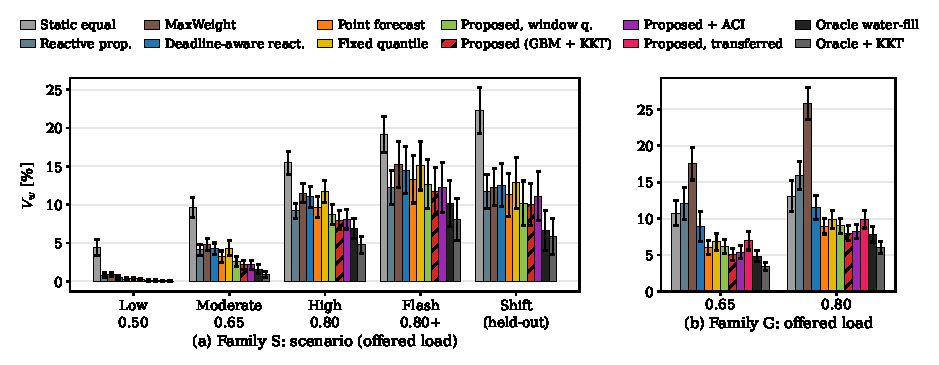
\includegraphics[width=0.92\textwidth]{paper_fig_overview}
\caption{Priority-weighted deadline-violation ratio $V_w$ (mean $\pm$ std over \nSeeds{} test seeds; lower is better) of all controllers in Table~\ref{tab:controllers}. (a) Family S, five scenarios; (b) Family G (3GPP TR~38.901 channel, FTP-3 / XR traffic), two loads. Hatched: proposed rule; black and dark grey: oracles (not implementable).}
\label{fig:overview}
\end{figure*}

\subsection{Family S: main comparison}
Fig.~\ref{fig:overview}(a) and Table~\ref{tab:main} report $V_w$ per scenario. The proposed rule is the best implementable controller in every scenario, and every paired reduction against a baseline is significant after Holm correction ($p < 0.01$), with the proposed rule winning \nSeeds{}/\nSeeds{} seeds against every baseline in every scenario except reactive proportional under flash crowds (\redoverloadburstsreactiveprop{}\,\% \redoverloadburstsreactivepropCI{}, \redoverloadburstsreactivepropWins{} seeds, $p < 0.05$). Against the point-forecast controller, which uses the same model, weights and information and differs only in using the median instead of the distribution, the reduction is \redPFmin{}--\redPFmax{}\,\% (95\,\% bootstrap intervals \redlowpointforecastCI{} at low load, \redshiftpointforecastCI{} under shift); this is the direct test of the value of representing uncertainty. Against the tuned deadline-aware reactive controller it is \redQAmin{}--\redQAmax{}\,\%. The tuned fixed-quantile controller is beaten everywhere: one global percentile over-reserves confident cells and under-reserves uncertain ones. The oracle + KKT reference shows what a perfect forecast would add to the same rule: \gapKKThigh{}\,\% of the proposed rule's $V_w$ at high load and \gapKKTshift{}\,\% under shift is forecast error, the remainder is the cost of committing budgets for 10~ms. Fig.~\ref{fig:demo} shows the mechanism on one LL cell: the proposed rule holds the \emph{smallest} mean budget of the three deadline-aware controllers (1.62 against 1.66 and 1.72~Mbit per slot) yet loses the fewest bits, because it raises the budget above the median only in epochs whose forecast distribution is wide.

\begin{figure}[t]
\centering
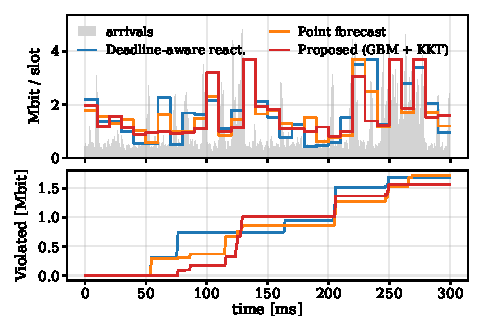
\includegraphics[width=0.94\columnwidth]{paper_fig_demo}
\caption{One low-latency cell of Family S at load 0.80. Top: fronthaul arrivals per slot (grey) and the budget held per 10-ms interval by three deadline-aware controllers. Bottom: cumulative deadline-violated bits.}
\label{fig:demo}
\end{figure}

\begin{table}[t]
\caption{Family S: $V_w$ (\%, mean $\pm$ std over \nSeeds{} test seeds; lower is better; bold = best implementable controller)}
\label{tab:main}
\centering
\scriptsize
\setlength{\tabcolsep}{1.2pt}
\begin{tabular}{lccccc}
\hline
Controller & Low 0.50 & Mod. 0.65 & High 0.80 & Flash & Shift \\
\hline
Static equal share & 4.45$\pm$1.05 & 9.65$\pm$1.36 & 15.46$\pm$1.51 & 19.15$\pm$2.34 & 22.31$\pm$2.99 \\
Reactive proportional & 0.83$\pm$0.27 & 4.11$\pm$0.69 & 9.20$\pm$0.99 & 12.27$\pm$2.23 & 11.70$\pm$2.24 \\
MaxWeight (drift) & 0.90$\pm$0.28 & 4.85$\pm$0.79 & 11.54$\pm$1.27 & 15.24$\pm$3.02 & 12.31$\pm$2.44 \\
Deadline-aware react. & 0.52$\pm$0.21 & 4.24$\pm$0.78 & 11.03$\pm$1.33 & 14.51$\pm$3.06 & 12.56$\pm$2.81 \\
Point forecast + WF & 0.27$\pm$0.17 & 3.23$\pm$0.73 & 9.70$\pm$1.34 & 13.33$\pm$3.09 & 11.30$\pm$2.81 \\
Fixed quantile + WF & 0.34$\pm$0.23 & 4.35$\pm$1.02 & 11.76$\pm$1.44 & 15.09$\pm$3.17 & 12.85$\pm$3.32 \\
Proposed, window q. & 0.25$\pm$0.13 & 2.57$\pm$0.64 & 8.72$\pm$1.34 & 12.67$\pm$3.19 & 10.22$\pm$2.88 \\
Proposed (GBM + KKT) & \textbf{0.15$\pm$0.13} & \textbf{2.15$\pm$0.60} & \textbf{8.00$\pm$1.27} & \textbf{11.76$\pm$3.08} & \textbf{10.04$\pm$2.71} \\
Proposed + ACI & 0.17$\pm$0.13 & 2.17$\pm$0.61 & 8.14$\pm$1.30 & 12.27$\pm$3.26 & 11.12$\pm$3.22 \\
\hline
Oracle water-fill & 0.07$\pm$0.10 & 1.62$\pm$0.56 & 6.89$\pm$1.28 & 10.16$\pm$2.96 & 6.69$\pm$2.60 \\
Oracle + KKT rule & 0.05$\pm$0.09 & 0.88$\pm$0.42 & 4.77$\pm$1.12 & 8.10$\pm$2.77 & 5.84$\pm$2.37 \\
\hline
\end{tabular}

\end{table}

\textbf{Where the gain comes from.} At high load the deadline-unaware controllers keep eMBB nearly clean (\meanhighreactivepropEMBB{}\,\% violations for reactive proportional) but let the LL cells lose \meanhighreactivepropLL{}\,\% of their bits. All deadline-aware controllers protect the LL cells (\meanhighproposedLL{}\,\% for the proposed rule) and pay with eMBB; within that group the proposed rule has the lowest eMBB loss (\meanhighproposedEMBB{}\,\% against \meanhighpointforecastEMBB{}\,\% for the point forecast) and the highest utilisation (\meanhighproposedUtil{}\,\%).

\textbf{Ablations.} The KKT rule fed with empirical window quantiles already beats every baseline; the learned model adds \redshiftproposedwindow{}\,\% under shift (\redshiftproposedwindowWins{} seeds) and up to \redlowproposedwindow{}\,\% in the nominal family, so most of the gain comes from the demand notion and the rule. Online conformal calibration is \redhighproposedcal{}\,\% worse at high load and \redshiftproposedcal{}\,\% under shift: in a coupled allocation LL misses are partly caused by the shortage split rather than by forecast bias, so the per-cell correction inflates LL reservations and starves eMBB.

\subsection{Family G: standards-based traffic and transfer}
\label{sec:tgpp}
Fig.~\ref{fig:overview}(b) and Table~\ref{tab:tgpp} repeat the comparison on the 3GPP-model family with its own forecaster and its own tuning. The main finding is reproduced: the proposed rule is the best implementable controller at both loads, winning \redtgpphighpointforecastWins{} seeds against every baseline at load \loadTgppHigh{}, with a reduction of \redtgpphighpointforecast{}\,\% against the point-forecast controller, \redtgpphighqueueaware{}\,\% against the deadline-aware reactive controller and \redtgpphighreactiveprop{}\,\% against reactive proportional. The traffic is harder in a different way: XR frames arrive every 16.7~ms and each 0.5-MByte FTP file occupies the whole cell for about 13 slots, so the eMBB class loses \meantgpphighoraclekktEMBB{}\,\% of its bits even under the oracle + KKT rule with 10-ms budgets, and the deadline-unaware controllers fall behind even static sharing. Unlike Family S, the proposed rule is here the best implementable controller also under the \emph{unweighted} ratio (\meantgpphighproposedUnw{}\,\% against \meantgpphighreactivepropUnw{}\,\% for reactive proportional), because the LL cells are small and periodic enough to be protected almost for free. The transferred variant, whose forecaster has never seen a 3GPP trace, under-reserves the LL cells (\meantgpphighproposedtransferLL{}\,\% against \meantgpphighproposedLL{}\,\%) and ends \redtgpphighproposedtransfer{}\,\% above the in-family model: still a usable allocation, but not better than an in-family point forecast. The gap to the oracle + KKT rule is \gapKKTtgpphigh{}\,\% at high load.

\begin{table}[t]
\caption{Family G: $V_w$ in \% at both loads (mean, $\pm$ std at high, \nSeedsTgpp{} seeds), LL / unweighted ratio at high load, and $\Delta$ = paired relative change of $V_w$ from the row controller to the proposed rule at high load (\%, negative = proposed better; seeds won of \nSeedsTgpp{}; $^{\ast}$/$^{\ast\ast}$: Holm-corrected Wilcoxon $p<0.05$/$0.01$)}
\label{tab:tgpp}
\centering
\scriptsize
\setlength{\tabcolsep}{3pt}
\begin{tabular}{lcccc}
\hline
Controller & Mod.\ 0.65 & High 0.80 & LL / unw. & $\Delta$ (wins) \\
\hline
Static equal share & 10.75 & 13.10$\pm$2.13 & 6.64 / 19.20 & -39 (20)$^{\ast\ast}$ \\
Reactive proportional & 12.05 & 15.94$\pm$1.93 & 16.96 / 15.01 & -50 (20)$^{\ast\ast}$ \\
MaxWeight (drift) & 17.51 & 25.79$\pm$2.15 & 32.17 / 19.75 & -69 (20)$^{\ast\ast}$ \\
Deadline-aware react. & 8.95 & 11.53$\pm$1.67 & 4.24 / 18.47 & -31 (20)$^{\ast\ast}$ \\
Point forecast + WF & 6.00 & 8.98$\pm$1.09 & 0.98 / 16.59 & -11 (20)$^{\ast\ast}$ \\
Fixed quantile + WF & 6.80 & 9.88$\pm$1.24 & 0.60 / 18.70 & -19 (20)$^{\ast\ast}$ \\
Proposed, window q. & 6.18 & 9.01$\pm$1.04 & 1.61 / 16.04 & -11 (20)$^{\ast\ast}$ \\
Proposed (GBM + KKT) & \textbf{5.08} & \textbf{8.01$\pm$0.99} & 1.28 / 14.40 & -- \\
Proposed + ACI & 5.41 & 8.27$\pm$0.98 & 1.12 / 15.06 & -3 (19)$^{\ast\ast}$ \\
Proposed, transferred & 6.99 & 9.89$\pm$1.18 & 5.29 / 14.27 & -19 (20)$^{\ast\ast}$ \\
\hline
Oracle water-fill & 4.82 & 7.85$\pm$1.06 & 0.23 / 15.09 & +2 (5)$^{\ast}$ \\
Oracle + KKT rule & 3.47 & 6.06$\pm$0.83 & 0.72 / 11.14 & +32 (0)$^{\ast\ast}$ \\
\hline
\end{tabular}

\end{table}

\subsection{The objective matters: unweighted ratio and priority weight}
\label{sec:weights}
The gain of every deadline-aware controller is a priority trade: fewer LL bits lost, more eMBB bits lost. Under the \emph{unweighted} violation ratio the proposed rule remains the best implementable controller in only \unwBestCount{} of the five Family S scenarios (low load): at high load reactive proportional loses fewer total bits (\meanhighreactivepropUnw{}\,\% against \meanhighproposedUnw{}\,\%) because it sacrifices the LL cells (\meanhighreactivepropLL{}\,\% of their bits) to serve eMBB volume. The weight sweep in Table~\ref{tab:sens} (last block; every controller is told the new $w^{\rm p}$, parameters stay tuned at $w_{\rm LL} = 3$) locates the crossover. In Family S at high load the proposed rule, given $w_{\rm LL} = 1$, matches proportional sharing (\wthighWoneproposed{} against \wthighWonereactiveprop{}\,\%) and beats it by \wthighWthreereactivepropRed{}\,\% at $w_{\rm LL} = 3$ and \wthighWfivereactivepropRed{}\,\% at 5; with a perfect forecast (oracle + KKT) the rule would win at every weight, so the loss at low weights is forecast error. In Family G at $w_{\rm LL} = 1$ the rule reaches \wttgpphighWoneproposed{}\,\% against \wttgpphighWonepointforecast{}\,\% for the point-forecast water-fill: XR and FTP demand is zero-inflated (often no frame or file falls into a horizon), and at a low common critical fractile the newsvendor solution reserves nothing beyond backlog for many cells, an all-or-nothing allocation that a median water-fill avoids (LL loss \wttgpphighWoneproposedLL{}\,\% against \wttgpphighWonepointforecastLL{}\,\%). At $w_{\rm LL} = 2$ the two tie and from 3 on the proposed rule leads (\wttgpphighWthreepointforecastRed{}\,\% and \wttgpphighWfivepointforecastRed{}\,\% against the point forecast). The method is therefore for operators who value a low-latency bit at least two to three times an eMBB bit.

\subsection{Operating regime: interval, delay, compression}
\label{sec:regime}
Table~\ref{tab:sens} varies, on the high-load scenario of Family S with forecasters retrained per setting, the control interval $T$ and the telemetry delay $\tau$, and on the moderate scenario the BFP mantissa width. \emph{Interval.} At $T = 2$~ms the proposed rule reduces $V_w$ by \sweepTfouroracle{}\,\% relative to even the oracle water-fill, which has a perfect point forecast: the allocation rule, not only the forecast, carries the gain (oracle + KKT reaches \sweepTfouroraclekktAbs{}\,\% against \sweepTfouroracleAbs{}\,\% for the oracle water-fill). At $T = 20$~ms, five times the LL deadline, reserving the LL peak rate for the whole interval wastes capacity and proportional sharing is better (\sweepTfourzeroreactiveprop{}\,\%). \emph{Delay.} All controllers degrade as state ages and the ordering is preserved, but the margin over proportional sharing shrinks from \delayTauzeroreactiveprop{}\,\% at $\tau = 0$ to \delayTauonezeroreactiveprop{}\,\% at $\tau = 5$~ms. \emph{Compression.} Mantissa widths of 6, 9, 12 and 14 bits rescale $\beta$ in \eqref{eq:beta} and move the offered load from 0.44 to 0.99 with the same user traffic. At 0.44 nothing is lost whatever the rule, at 0.65 the proposed rule loses about half as much as the reactive controllers, at 0.86 proportional sharing is slightly better on $V_w$, and at 0.99 no rule helps. Compression selects the load regime; deadline-aware allocation matters between about 0.5 and 0.8 and should hand over to proportional sharing or stronger compression above that.

\begin{table}[t]
\caption{Sensitivity on Family S: $V_w$ (\%, means over \nSeedsSweep{}/\nSeedsDelay{}/\nSeedsComp{}/\nSeedsWeights{} seeds; bold = best implementable)}
\label{tab:sens}
\centering
\scriptsize
\begin{tabular}{lcccc}
\hline
\multicolumn{5}{l}{\textit{Control interval $T$ (high)}} \\
Controller & 2 ms & 5 ms & 10 ms & 20 ms \\
\hline
Reactive proportional & 3.91 & 7.42 & 8.91 & \textbf{11.80} \\
Deadline-aware reactive & 7.89 & 10.20 & 10.78 & 15.84 \\
Point forecast + WF & 6.57 & 7.53 & 9.46 & 14.08 \\
\textbf{Proposed (GBM + KKT)} & \textbf{3.07} & \textbf{5.07} & \textbf{7.71} & 13.15 \\
Oracle water-fill & 6.89 & 6.01 & 6.63 & 10.83 \\
Oracle + KKT rule & 1.91 & 2.74 & 4.52 & 8.14 \\
\hline
\multicolumn{5}{l}{\textit{Telemetry delay $\tau$ (high)}} \\
Controller & 0 ms & 1 ms & 2.5 ms & 5 ms \\
\hline
Reactive proportional & 8.16 & 8.91 & 9.86 & 11.30 \\
Deadline-aware reactive & 9.89 & 10.78 & 11.90 & 13.93 \\
Point forecast + WF & 8.45 & 9.46 & 10.51 & 12.45 \\
\textbf{Proposed (GBM + KKT)} & \textbf{6.85} & \textbf{7.71} & \textbf{8.77} & \textbf{11.07} \\
\hline
\multicolumn{5}{l}{\textit{BFP width / load (moderate)}} \\
Controller & 6b/0.44 & 9b/0.65 & 12b/0.86 & 14b/0.99 \\
\hline
Reactive proportional & 0.22 & 3.90 & \textbf{11.37} & \textbf{17.29} \\
Deadline-aware reactive & 0.18 & 4.02 & 13.84 & 20.38 \\
Point forecast + WF & 0.15 & 3.00 & 12.50 & 19.16 \\
\textbf{Proposed (GBM + KKT)} & \textbf{0.11} & \textbf{1.96} & 12.01 & 20.81 \\
\hline
\multicolumn{5}{l}{\textit{LL priority weight $w_{\mathrm{LL}}$ (high)}} \\
Controller & 1 & 2 & 3 & 5 \\
\hline
Reactive proportional & \textbf{6.55} & \textbf{8.13} & 9.20 & 10.56 \\
MaxWeight (drift) & 7.38 & 9.96 & 11.54 & 13.38 \\
Deadline-aware reactive & 7.75 & 10.08 & 11.03 & 11.69 \\
Point forecast + WF & 6.77 & 8.90 & 9.70 & 10.57 \\
\textbf{Proposed (GBM + KKT)} & 6.58 & 8.35 & \textbf{8.00} & \textbf{6.93} \\
Oracle water-fill & 4.86 & 5.97 & 6.89 & 8.29 \\
Oracle + KKT rule & 4.86 & 5.68 & 4.77 & 3.63 \\
\hline
\end{tabular}

\end{table}

\subsection{Robustness to miscalibration}
\label{sec:robust}
To test Proposition~\ref{prop:robust} every forecast quantile level is shifted by $\epsilon \in \{-0.3, -0.2, \dots, 0.3\}$ before allocation, a Kolmogorov distance of $|\epsilon|$ (\nSeedsMisc{} seeds). Under-reserving ($\epsilon < 0$) is almost harmless (\mischighUnder{}\,\% at $\epsilon = -0.3$ against \mischighBase{}\,\% at $\epsilon = 0$ at high load): when the link constraint binds, a common shift of all levels is largely absorbed by $\lambda^\ast$, which equalises weighted levels rather than using them absolutely. Over-reserving degrades gradually, to \mischighWorst{}\,\% at $\epsilon = +0.3$ (\mischighWorstRel{}\,\% relative), because the upper quantiles saturate at the last knot and the rule loses the tail resolution that distinguishes cells. Even then the rule matches the point-forecast controller (\mischighpointforecast{}\,\%) and beats the deadline-aware reactive one (\mischighqueueaware{}\,\%); the degradation is bounded and roughly linear in $\epsilon$, as predicted.

\section{Discussion, Limitations and Conclusion}
\label{sec:limits}
When budgets must be committed before the traffic is known, turning a forecast \emph{distribution} of deadline-feasible demand into per-cell budgets through the KKT rule reduces priority-weighted deadline violations compared with point forecasts, tuned global quantiles, queue-based and deadline-aware reactive controllers, on two unrelated traffic families and under distribution shift, cross-family transfer and forecast miscalibration. The claim holds in a stated regime: the objective must value the low-latency class (at $w_{\rm LL} \le 2$ the simpler controllers are as good or better); control interval and telemetry age must stay within a few times the shortest deadline; above a load of about 0.85 no allocation rule helps and compression or capacity must; and per-stream conformal calibration harms the coupled allocation. Limitations: both families are simulated; Family G uses a round-robin scheduler, flat fading and a fixed rank; the link is a budget-enforced pipe without a switch-queue model; each cell carries one class; HARQ, uplink and the signal-quality cost of compression are not modelled. Next steps are validation on measured per-cell PRB traces and a joint controller for compression and allocation.

\begin{thebibliography}{00}
\bibitem{oran_cus} O-RAN Alliance WG4, ``Control, user and synchronization plane specification,'' O-RAN.WG4.CUS.0, 2024.
\bibitem{polese2023} M. Polese, L. Bonati, S. D'Oro, S. Basagni, and T. Melodia, ``Understanding O-RAN: Architecture, interfaces, algorithms, security, and research challenges,'' \emph{IEEE Commun. Surveys Tuts.}, vol. 25, no. 2, pp. 1376--1411, 2023.
\bibitem{larsen2019} L. M. P. Larsen, A. Checko, and H. L. Christiansen, ``A survey of the functional splits proposed for 5G mobile crosshaul networks,'' \emph{IEEE Commun. Surveys Tuts.}, vol. 21, no. 1, pp. 146--172, 2019.
\bibitem{perez2018} G. O. P\'erez, J. A. Hern\'andez, and D. Larrabeiti, ``Fronthaul network modeling and dimensioning meeting ultra-low latency requirements for 5G,'' \emph{J. Opt. Commun. Netw.}, vol. 10, no. 6, pp. 573--581, 2018.
\bibitem{wang2017} L. Wang and S. Zhou, ``On the fronthaul statistical multiplexing gain,'' \emph{IEEE Commun. Lett.}, vol. 21, no. 5, pp. 1099--1102, 2017.
\bibitem{lagen2022} S. Lag\'en, X. Gelabert, A. Hansson, M. Requena, and L. Giupponi, ``Fronthaul compression control for shared fronthaul access networks,'' \emph{IEEE Commun. Mag.}, vol. 60, no. 4, pp. 70--76, 2022.
\bibitem{bega2019} D. Bega, M. Gramaglia, M. Fiore, A. Banchs, and X. Costa-P\'erez, ``DeepCog: Cognitive network management in sliced 5G networks with deep learning,'' in \emph{Proc. IEEE INFOCOM}, 2019.
\bibitem{bega2020} D. Bega, M. Gramaglia, M. Fiore, A. Banchs, and X. Costa-P\'erez, ``AZTEC: Anticipatory capacity allocation for zero-touch network slicing,'' in \emph{Proc. IEEE INFOCOM}, 2020.
\bibitem{sciancalepore2017} V. Sciancalepore, K. Samdanis, X. Costa-P\'erez, D. Bega, M. Gramaglia, and A. Banchs, ``Mobile traffic forecasting for maximizing 5G network slicing resource utilization,'' in \emph{Proc. IEEE INFOCOM}, 2017.
\bibitem{kavehmadavani2023} F. Kavehmadavani, V.-D. Nguyen, T. X. Vu, and S. Chatzinotas, ``Intelligent traffic steering in beyond 5G open RAN based on LSTM traffic prediction,'' \emph{IEEE Trans. Wireless Commun.}, vol. 22, no. 11, pp. 7727--7742, 2023.
\bibitem{kasuluru2024} V. Kasuluru, L. Blanco, C. J. Vaca-Rubio, and E. Zeydan, ``On the impact of PRB load uncertainty forecasting for sustainable open RAN,'' arXiv:2407.14400, 2024.
\bibitem{cohen2023} K. M. Cohen, S. Park, O. Simeone, P. Popovski, and S. Shamai, ``Guaranteed dynamic scheduling of ultra-reliable low-latency traffic via conformal prediction,'' \emph{IEEE Wireless Commun. Lett.}, vol. 12, no. 2, pp. 296--300, 2023.
\bibitem{gibbs2021} I. Gibbs and E. Cand\`es, ``Adaptive conformal inference under distribution shift,'' in \emph{Proc. NeurIPS}, 2021.
\bibitem{neely2010} M. J. Neely, \emph{Stochastic Network Optimization with Application to Communication and Queueing Systems}. Morgan \& Claypool, 2010.
\bibitem{hadley1963} G. Hadley and T. M. Whitin, \emph{Analysis of Inventory Systems}. Englewood Cliffs, NJ: Prentice-Hall, 1963.
\bibitem{leboudec2001} J.-Y. Le Boudec and P. Thiran, \emph{Network Calculus: A Theory of Deterministic Queuing Systems for the Internet}. Springer, 2001.
\bibitem{willinger1997} W. Willinger, M. S. Taqqu, R. Sherman, and D. V. Wilson, ``Self-similarity through high-variability: Statistical analysis of Ethernet LAN traffic at the source level,'' \emph{IEEE/ACM Trans. Netw.}, vol. 5, no. 1, pp. 71--86, 1997.
\bibitem{colo_ran} M. Polese, L. Bonati, S. D'Oro, S. Basagni, and T. Melodia, ``ColO-RAN: Developing machine learning-based xApps for open RAN closed-loop control on programmable experimental platforms,'' \emph{IEEE Trans. Mobile Comput.}, vol. 22, no. 10, pp. 5787--5800, 2023.
\bibitem{tr38901} 3GPP, ``Study on channel model for frequencies from 0.5 to 100 GHz,'' TR 38.901, 2022.
\bibitem{tr36942} 3GPP, ``E-UTRA; RF system scenarios,'' TR 36.942, 2022.
\bibitem{ts38214} 3GPP, ``NR; Physical layer procedures for data,'' TS 38.214, 2022.
\bibitem{tr36814} 3GPP, ``Further advancements for E-UTRA physical layer aspects,'' TR 36.814, 2017.
\bibitem{tr38838} 3GPP, ``Study on XR evaluations for NR,'' TR 38.838, 2021.
\end{thebibliography}

\end{document}
